\subsection{Vision Transformer}
\label{sec:vision_transformer}

\begin{figure*}[htbp]
\centering
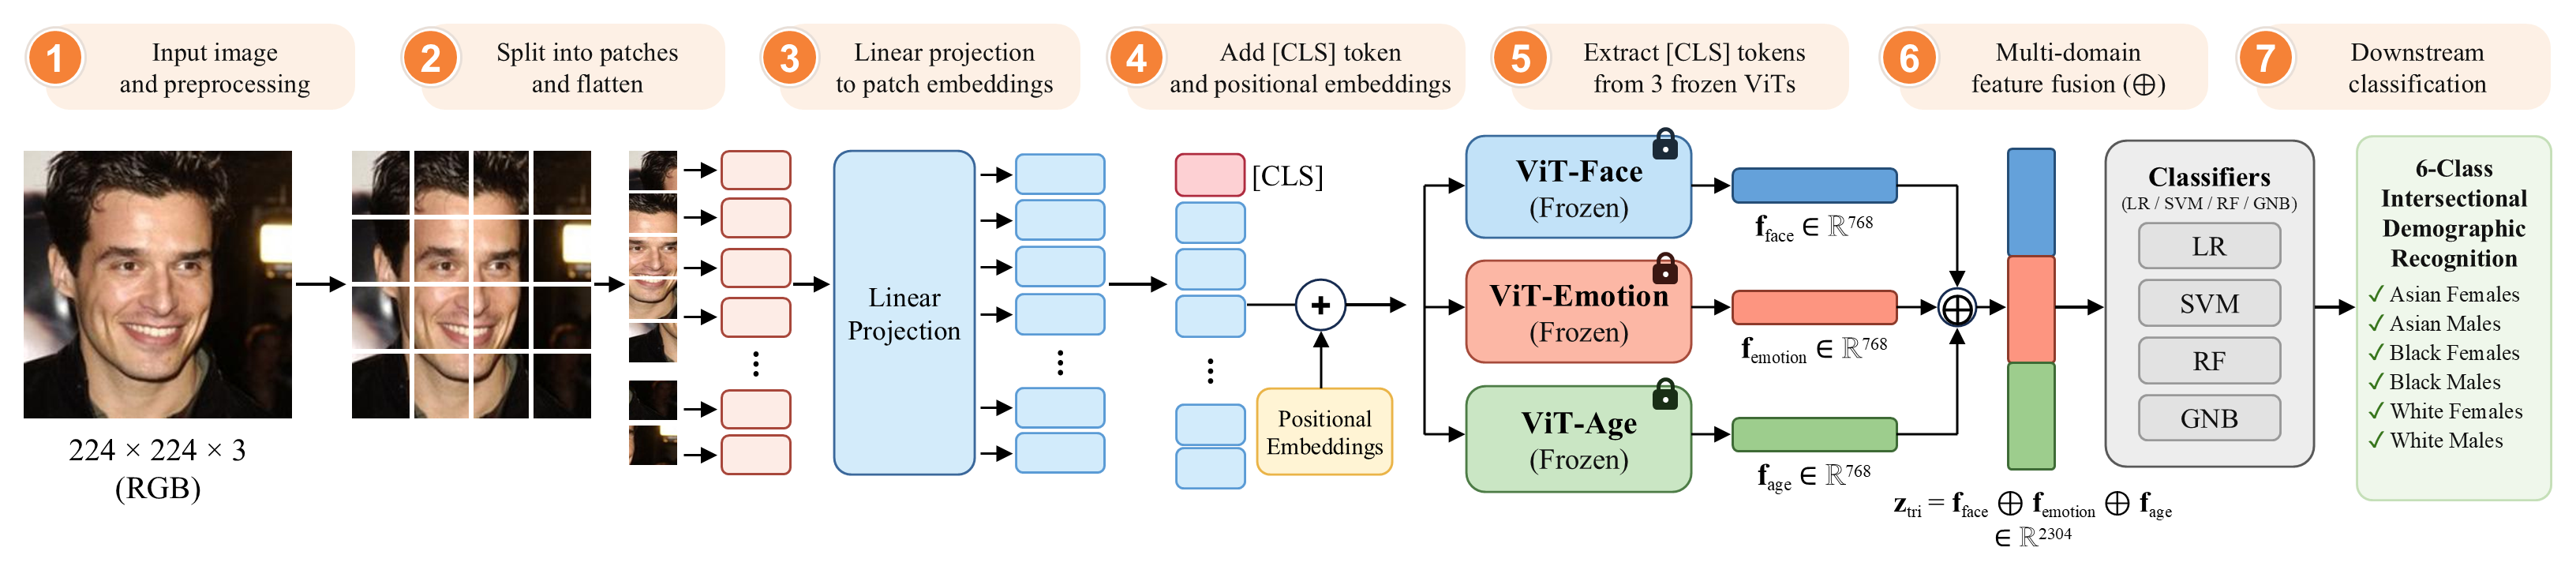
\includegraphics[width=\textwidth]{vit_v2.2.png}
\caption{Architecture of Multi-Domain ViT Feature Extraction and Fusion.}
\label{fig:3}
\end{figure*}

The visual feature extraction architecture adopts the standard ViT model mapped into the computational flow in Figure~\ref{fig:3}~\cite{ref26}. In Stage~1, an input image of 224 $\times$ 224 pixels ($C = 3$ channels) is processed, and then in Stage~2 partitioned into $N = 196$ non-overlapping patches of size $P \times P$ ($P = 16$). The patches are flattened into $\mathbf{x}_p \in \mathbb{R}^{P^2 \cdot C}$ and in Stage~3 projected via a linear matrix $\mathbf{E} \in \mathbb{R}^{(P^2 \cdot C) \times D}$ into a latent space of $D = 768$. In Stage~4, the patch vectors are combined with a class token $\mathbf{x}_{\text{class}} \in \mathbb{R}^D$ and positional encodings $\mathbf{E}_{\text{pos}} \in \mathbb{R}^{(N+1) \times D}$ according to \eqref{eq:5}~\cite{ref27}. The sequence $\mathbf{z}_0$ is passed into $L = 12$ transformer encoder layers, where features are processed through MHSA and a GeLU-activated MLP according to \eqref{eq:6}~\cite{ref28}. Stage~1 to 4 are depicted once for visual efficiency, but proceed independently in each backbone in Stage~5~\cite{ref29}.

\begin{equation}
\mathbf{z}_0 = [\mathbf{x}_{\text{class}}; \, \mathbf{x}_p^1\mathbf{E}; \, \dots; \, \mathbf{x}_p^N\mathbf{E}] + \mathbf{E}_{\text{pos}}
\label{eq:5}
\end{equation}

\begin{equation}
\mathbf{z}'_\ell = \text{MHSA}(\text{LN}(\mathbf{z}_{\ell-1})) + \mathbf{z}_{\ell-1}, \quad \mathbf{z}_\ell = \text{MLP}(\text{LN}(\mathbf{z}'_\ell)) + \mathbf{z}'_\ell
\label{eq:6}
\end{equation}

To obtain complementary visual representations, this framework utilizes three frozen pre-trained ViT-Base backbone models (frozen weights), all fine-tuned from google/\allowbreak vit-base-patch16-224-in21k. The first model is ViT-Face (skutaada/\allowbreak VIT-VGGFace, version e85f0c9), fine-tuned on the VGGFace2 corpus to map static biometric craniofacial geometry. The second model is ViT-Emotion (dima806/\allowbreak facial\_emotions\_\allowbreak image\_detection, version 747cf16), based on the FER-2013 corpus to extract dynamic affective expressions. The third model is ViT-Age (dima806/\allowbreak facial\_age\_\allowbreak image\_detection, version ad35933), based on a combined corpus of UTKFace and IMDB-WIKI for biological aging estimation. All models share a ViT-Base/16 architecture with a latent dimension of 768 and 12 encoder layers. Input RGB images of 224 $\times$ 224 pixels are processed via AutoImageProcessor with uniform normalization $\mu = \sigma = [0.5, 0.5, 0.5]$ per channel and accelerated via in-memory processor caching for computational efficiency and reproducibility.

\begin{table}[htbp]
\caption{Multi-Domain Feature Fusion and Systematic Ablation Configurations.}
\label{tab:2}
\label{tab:II}
\centering
\footnotesize
\setlength{\tabcolsep}{3.5pt}
\begin{tabular}{clcc}
\toprule
\# & Feature Scheme & Category & Dimension \\
\midrule
1 & Face & Single-Domain & 768 \\
2 & Emotion & Single-Domain & 768 \\
3 & Age & Single-Domain & 768 \\
4 & Emotion $\oplus$ Face & Dual-Domain & 1,536 \\
5 & Face $\oplus$ Age & Dual-Domain & 1,536 \\
6 & Emotion $\oplus$ Age & Dual-Domain & 1,536 \\
7 & Face $\oplus$ Emotion $\oplus$ Age & Tri-Domain (Proposed) & 2,304 \\
\bottomrule
\end{tabular}
\end{table}

In Stage~5, high-level latent feature representations are extracted in parallel from the three frozen ViT backbones via the $[\text{CLS}]$ class token activations at the final encoder layer ($\ell = 12$). The output vectors are standardized via a final Layer Normalization to yield the representation $\mathbf{f}_{\text{domain}} \in \mathbb{R}^{768}$ according to \eqref{eq:7}, where $\mathbf{z}_{12}^0$ denotes the first token of the 12th layer without gradient updates. Subsequently, in Stage~6, the three representations are merged via direct concatenation fusion $\oplus$ into a tri-domain vector $\mathbf{z}_{\text{tri}} \in \mathbb{R}^{2304}$ based on \eqref{eq:8}, unifying craniofacial information $\mathbf{f}_{\text{face}}$, affective features $\mathbf{f}_{\text{emotion}}$, and biological age $\mathbf{f}_{\text{age}}$. This representation is forwarded to Stage~7 for downstream six-class intersectional classification. The methodological novelty centers on an efficient complementary multi-domain fusion evaluation framework without retraining or fine-tuning computation, which is systematically evaluated across the seven feature configurations in Table~\ref{tab:2}.

\begin{equation}
\mathbf{f}_{\text{domain}} = \text{LN}(\mathbf{z}_{12}^0) \in \mathbb{R}^{768}
\label{eq:7}
\end{equation}

\begin{equation}
\mathbf{z}_{\text{tri}} = \mathbf{f}_{\text{face}} \oplus \mathbf{f}_{\text{emotion}} \oplus \mathbf{f}_{\text{age}} \in \mathbb{R}^{2304}
\label{eq:8}
\end{equation}
